\chapter{Identical particles}

\section{Two-particle system}
For a single particle, $\Psi \left( \mathbf{r},t \right)$ is a function of the spatial coordinate and time (we will ignore spin).
For two-particle system the wave function is $\Psi \left( \mathbf{r}_1, \mathbf{r}_2, t \right)$.
It evolves with the Schr\"odinger equation with the Hamiltonian
\begin{equation}
  \label{eq:5-1}
 H = - \frac{\hbar^{2}}{2m_{1}} \nabla_1^2 - \frac{\hbar^{2}}{2m_{2}} \nabla_2^2 + V \left( \mathbf{r}_1,\mathbf{r}_2,t \right).
\end{equation}

Typically, the interaction potential depends only the vector $\mathbf{r} \equiv \mathbf{r}_1 - \mathbf{r}_2$ between the two particles.
We can change the variable to $\mathbf{r}$ and $\mathbf{R} \equiv \frac{m_{1} \mathbf{r}_1 + m_2 \mathbf{r}_2}{m_1+m_2}$.
Relate to the old coordinate, we have $\mathbf{r}_{1,2} = \mathbf{R} \pm \mathbf{r} \frac{\mu}{m_{1,2}}$, and $\nabla_{1,2} = \frac{\mu}{m_{2,1}} \nabla_R \pm \nabla_{r}$ where
\begin{equation}
  \label{eq:5-2}
 \mu \equiv \frac{m_1 m_2}{m_1 + m_2}
\end{equation}
is the \textbf{reduced mass} of the system.
The Shr\"odinger equation becomes
\begin{equation}
  \label{eq:5-3}
 - \frac{\hbar^{2}}{2 \left( m_1 + m_2 \right)}  \nabla^2_R \psi - \frac{\hbar^{2}}{2\mu} \nabla^2_r \psi + V \left( \mathbf{r} \right) \psi = E\psi.
\end{equation}
We can further separate the variables, $\psi \left( \mathbf{R}, \mathbf{r} \right) = \psi_R \left( \mathbf{R} \right) \psi_r \left( \mathbf{r} \right)$ to see that they are two single particle problem.

\subsection{Bosons and Fermions}
Suppose there are two particles and they can be represented in the way of simple product\footnote{In \textbf{entangled states}, you can not decomposed in that way. If particle one is in state $a$ and particle two is in state $b$, then the two-particle state is a product. The simplest example of entangled state is the singlet spin configuration in Eq.~\eqref{eq:4-126}. You can not tell the state of particle one by itself, because it is ``entangled'' with the state of particle two. If $2$ is measured, and found to be spin up, then $1$ is spin down, but if $2$ is spin down, then $1$ is spin up.}
\begin{equation}
  \label{eq:5-4}
  \psi \left( \mathbf{r}_1, \mathbf{r}_2 \right)  = \psi_a \left( \mathbf{r}_1 \right) \psi_b \left( \mathbf{r}_2 \right).
\end{equation}
Of course, this assumes that we can tell the particles apart---otherwise it wouldn't make any sense to claim that number $1$ is in state $\psi_a$ and number $2$ is in state $\psi_b$; all we could say is that one of them is in the state $\psi_a$ and the other is in state $\psi_b$, but we wouldn't know which is which.
\marginnote{Some discussion from \href{https://physics.stackexchange.com/questions/405155/are-identical-particles-always-entangled-even-when-not-interacting}{stackexchange}:

Entanglement is only a meaningful concept when there is a well-defined notion of subsystems, which generally means spatially separated subsystems. Indeed, the notion of "product state" (or its converse, "entangled state") is only meaningful relative to a given tensor product decomposition of the Hilbert space, which implicitly defines a splitting into subsystems. Hence, it is not obvious that indistinguishable particles with an (anti-)symmetrised wavefunction can be truly regarded as entangled subsystems.

Nevertheless, \href{https://arxiv.org/abs/1312.4311}{Killoran, Cramer and Plenio} showed that this is indeed a genuine form of entanglement. That is, the entanglement formally associated with the symmetrised wave function of a system of indistinguishable bosons can be extracted into the equivalent amount of entanglement (asymptotically) between distinguishable modes.
I believe a similar result was found also for fermions by \href{https://arxiv.org/abs/quant-ph/0608141}{Cavalcanti et al}.
}
This is what happened, since all electrons are utterly identical unlike classical objects.

Quantum mechanics neatly accommodates the existence of particles that are \textit{indistinguishable in principle:} We simply construct a wave function that is \textit{noncommittal} as to which particle is in which state.
There are actually two ways to do it
\begin{equation}
  \label{eq:5-5}
 \psi_{\pm} \left( \mathbf{r}_1, \mathbf{r}_2 \right) = A \left[ \psi_a \left( \mathbf{r}_1 \right) \psi_b \left( \mathbf{r}_2 \right) \pm \psi_b \left( \mathbf{r}_1 \right) \psi_a \left( \mathbf{r}_2 \right) \right] .
\end{equation}
Thus the theory admits two kinds of identical particles: \textbf{bosons} (plus sign with integer spin) and \textbf{fermions} (minus sign with half integer spin).
This connection between \textbf{spin and statistics} can be proved in relativistic quantum mechanics; in non-relativistic theory it is taken as an axiom.

It follows, in particular, that \textit{two identical fermions can not occupy the same state}.
This is the famous \textbf{Pauli exclusion principle}.
There is a more general way to formulate the problem.
Let us define the \textbf{exchange operator}, $P$, which interchanges the two particles:
\begin{equation}
  \label{eq:5-6}
 P f lr(r_1,r_2) = f lr(r_2,r_1) .
\end{equation}
Clearly, $P^2=1$, and it follows that the eigenvalues of $P$ are $\pm 1$.
Now, if the two particles are identical, the Hamiltonian must treat them the same: $m_1=m_2$ and $V \left( r_1,r_2 \right)=V \left( r_2,r_1 \right)$.
This suggest that $P$ and $H$ are compatible observables
\begin{equation}
  \label{eq:5-7}
  \left[ P,H \right]=0,
\end{equation}
and hence we can find a complete set of functions that are simultaneous eigenstates of both.
That is to say, we can find solutions to the Schr\"odinger equation that are either symmetric or antisymmetric under exchange:
\begin{equation}
  \label{eq:5-8}
 \psi \left( r_1, r_2 \right) = \pm \psi \left( r_2, r_1 \right) .
\end{equation}
Moreover, if a system starts our in such state, it will remain in a such state.
For identical particles the wave function is not merely \textit{allowed}, but \textit{required} to satisfy Eq.~\eqref{eq:5-8}, with the plus sign for bosons, and minus sign for fermions.

\subsection{Exchange force}
Suppose on particle is in state $\psi_a \left( x \right)$, and the other is in state $\psi_b \left( x \right)$, and these two states are orthogonal and normalized.
If the two particle are distinguishable, and number $1$ is in the state $\psi_a$, then the combined wave function is
\begin{equation}
  \label{eq:5-9}
  \psi \left( x_1,x_2 \right) = \psi_a \left( x_1 \right) \psi_b \left( x_2 \right);
\end{equation}
if they are identical particles, the composite wave function is
\begin{equation}
  \label{eq:5-10}
 \psi_{\pm} \left( x_1,x_2 \right) = \frac{1}{\sqrt{2}} \left[ \psi_a \left( x_1 \right) \psi_b \left( x_2 \right) \pm \psi_b \left( x_1 \right) \psi_a \left( x_2 \right) \right].
\end{equation}
We will calculate the expectation value of the square of the separation distance between the two particles,
\begin{equation}
  \label{eq:5-11}
 \expval{\left( x_1 - x_2 \right)^2} = \expval{x_1^2} + \expval{x_2^2} - 2\expval{x_1x_2}.
\end{equation}

\textbf{Case 1: Distinguishable particles}. For the wavefunction in Eq.~\eqref{eq:5-9},
\begin{equation*}
  \expval{ x_1^2 } = \int x_1^2 \abs{ \psi_a \left( x_1 \right) }^2 \dd x_1 \int \abs{\psi_b \left( x_2 \right)} \dd x_{2} = \expval{x^2}_{a}
\end{equation*}
With similar procedure, we have the result:
\begin{equation}
  \label{eq:5-12}
   \expval{\left( x_1 - x_2 \right)^2}_d = \expval{x_1^2}_a + \expval{x_2^2}_b - 2\expval{x_1}_a\expval{x_2}_b.
\end{equation}

\textbf{Case 2: Identical particles.} For the wave function in Eq.~\eqref{eq:5-10},
\begin{align*}
  \expval{x_1^2} &= \frac{1}{2} \Big[ \int x_1^2 \abs{ \psi_a \left( x_1 \right) }^2 \dd x_1 \int \abs{\psi_b \left( x_2 \right)} \dd x_{2}\\
                 &+  \int x_1^2 \abs{ \psi_b \left( x_1 \right) }^2 \dd x_1 \int \abs{\psi_a \left( x_2 \right)} \dd x_{2}\\
                 &\pm \int x_1^2 \psi_a \left( x_1 \right)^{*} \psi_b \left( x_1 \right) \dd x_1 \int \psi_b \left( x_2 \right)^{*} \psi_a \left( x_2 \right) \dd x_{2}\\
                 &\pm \int x_1^2 \psi_b \left( x_1 \right)^{*} \psi_a \left( x_1 \right) \dd x_1 \int \psi_a \left( x_2 \right)^{*} \psi_b \left( x_2 \right) \dd x_{2} \Big] \\
                 &= \frac{1}{2} \left[ \expval{x^2}_a + \expval{x^2}_b \pm 0 \pm 0 \right]
\end{align*}
Since particle are identical you can not tell them apart, we have same result for $\expval{x_2^{2}}$.
But for the rest part,
\begin{align*}
  \expval{x_1 x_2} &= \frac{1}{2} \Big[ \int x_1 \abs{ \psi_a \left( x_1 \right) }^2 \dd x_1 \int x_2 \abs{\psi_b \left( x_2 \right)} \dd x_{2}\\
                   &+  \int x_1 \abs{ \psi_b \left( x_1 \right) }^2 \dd x_1 \int x_2 \abs{\psi_a \left( x_2 \right)} \dd x_{2}\\
                   &\pm \int x_1 \psi_a \left( x_1 \right)^{*} \psi_b \left( x_1 \right) \dd x_1 \int x_2 \psi_b \left( x_2 \right)^{*} \psi_a \left( x_2 \right) \dd x_{2}\\
                   &\pm \int x_1 \psi_b \left( x_1 \right)^{*} \psi_a \left( x_1 \right) \dd x_1 \int x_2 \psi_a \left( x_2 \right)^{*} \psi_b \left( x_2 \right) \dd x_{2} \Big] \\
                   &= \expval{x}_a \expval{x}_b \pm \abs{ \expval{x}_{ab} }^{2},
\end{align*}
where
\begin{equation}
  \label{eq:5-13}
 \expval{x}_{ab} \equiv \int x \psi_a \left( x \right)^{*} \psi_b \left( x \right) \dd x.
\end{equation}
Evidently, we have the result:
\begin{equation}
  \label{eq:5-14}
   \expval{\left( x_1 - x_2 \right)^2}_\pm = \expval{x_1^2}_a + \expval{x_2^2}_b - 2\expval{x_1}_a\expval{x_2}_b \mp 2 \abs{\expval{x}_{ab}}^{2}.
\end{equation}

Comparing Eq.~\eqref{eq:5-12} and Eq.~\eqref{eq:5-14}, we see that the difference resides in the final term:
\begin{equation}
  \label{eq:5-15}
 \expval{ \left( \Delta x \right)^2 }_{\pm} = \expval{ \left( \Delta x \right)^2 }_d \mp 2 \abs{ \expval{x}_{ab} }^{2}.
\end{equation}
Identical bosons tend to be somewhat closer together, and identical fermions somewhat further apart, than distinguishable particle in the same two states.
Notice that $\expval{x}_{ab}$ vanishes unless the two wave functions actually overlap.
As a \textit{practical} matter, therefore, it is okay to pretend that electrons with non-overlapping wave functions are distinguishable.

The \textit{interesting} case is when there is some overlap of the wave function.
The system behaves as through there were a ``force of attraction'' between identical bosons, pulling them closer together, and a ``force of repulsion'' between identical fermions, pushing them apart.
We call it an \textbf{exchange force}, although it is not really a force at all---no physical agency is pushing on the particles; rather, it is a purely \textit{geometrical} consequence of the symmetrization requirement.
It is also a strictly quantum mechanical phenomenon, with no classical counterpart.

There has profound consequences.
Considering the hydrogen molecule $H_{2}$.
Roughly speaking, the ground state consists of one electron in the atomic ground state, Eq.~\eqref{eq:4-53}, centered at nucleus $1$, and one electron in the atomic ground state centered at nucleus $2$.
If electrons where \textbf{bosons}, the symmetrization requirement would tend to concentrate the electrons toward the middle, between the two protons, and the resulting accumulation of negative charge  would attract the protons inward, accounting for the \textbf{covalent bound} as shown in Fig.~\ref{fig:5-1}.
Unfortunately, electron are not bosons, they are fermions, and this means that the concentration of negative charge should actually be shifted to the wings, tearing the molecule apart.
\begin{figure}[t]
  \centering
  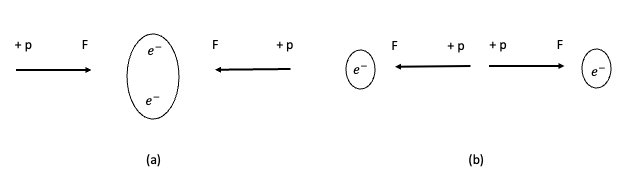
\includegraphics[width=0.75\textwidth]{fig/fig5-1.png}
  \label{fig:5-1}
  \caption{Schematic picture of the covalent bond: (a) Symmetric configuration produce attractive force. (b) Antisymmetric configuration produce repulsive force.}
\end{figure}

However, this is the conclusion when the spin is ignored.
The complete state of the electron includes not only its position wave function, but also a spinor, describing the orientation of the spin.
When we put together the two-electron state, it is the \textbf{whole works}, not just the spatial part, that has to be antisymmetric with respect to exchange.
Now, a glance back at the composite spin states Eq.~\eqref{eq:4-125} and Eq.~\eqref{eq:4-126} reveals that the singlet combination is antisymmetric and hence would have to be joined with a symmetric spatial function, whereas the three triplet states are all symmetric and would require an antisymmetric spatial function.
Evidently, then, the singlet state should lead to \textit{binding}, and the triplet to \textit{antibonding}.
Sure enough, the chemists tell us that covalent bonding requires the two electrons to occupy the singlet state, with total spin zero.

\section{Atoms}
A neutral atom, of atomic number $Z$, consists of a heavy nucleus, with electric charge $Ze$, surrounded by $Z$ electrons.
The Hamiltonian for the system\footnote{We are assuming the nucleus is stationary. The nucleus is so much more massive than the electrons that the correction is extremely small even in the case of hydrogen and it is smaller still for the heavier atoms.}
\begin{equation}
  \label{eq:5-16}
 H = \sum_{j=1}^Z \left\{ - \frac{\hbar^{2}}{2m} \nabla^2_j - \left( \frac{1}{4\pi \epsilon_{0}} \right)  \frac{Z e^{2}}{r_{j}}\right\} + \frac{1}{2} \left( \frac{1}{4 \pi \epsilon_{0}} \right) \sum_{j \neq k}^Z \frac{e^{2}}{\abs{\mathbf{r}_j - \mathbf{r}_k}}.
\end{equation}
The term in curly brackets represents the kinetic plus potential energy of the $j$th electron, in the electric field of the nucleus; the second sum is the potential energy associated with the mutual repulsion of the electrons.
The problem is to solve Schr\"odinger's equation,
\begin{equation}
  \label{eq:5-17}
 H \psi = E \psi,
\end{equation}
for the wave function $\psi \left( \mathbf{r}_1, \ldots, \mathbf{r}_Z \right)$.
Because electrons are identical, for the complete state,
\begin{equation}
  \label{eq:5-18}
  \psi \left( \mathbf{r}_1, \ldots, \mathbf{r}_Z \right) \chi \left( \mathbf{s}_1, \ldots, \mathbf{s}_{Z} \right),
\end{equation}
should be antisymmetric with respect to interchange of any two electrons.

The Schr\"odinger equation with Hamiltonian in Eq.~\eqref{eq:5-16} can not be solved exactly.
Some qualitative features will be discussed here.

\subsection{Helium}
After the hydrogen, the simplest atom is helium ($Z=2$).
The Hamiltonian,
\begin{equation}
  \label{eq:5-19}
  H = \left\{ - \frac{\hbar^{2}}{2m} \nabla_1^2 - \frac{1}{4\pi \epsilon_{0}} \frac{2e^{2}}{r_{1}} \right\} +  \left\{ - \frac{\hbar^{2}}{2m} \nabla_2^2 - \frac{1}{4\pi \epsilon_{0}} \frac{2e^{2}}{r_{2}} \right\} + \frac{1}{4\pi\epsilon_{0}} \frac{e^{2}}{\abs{\mathbf{r}_1- \mathbf{r}_{2}}},
  \end{equation}
consists of two hydrogenic Hamiltonians.
If we simply \textit{ignore} the last interaction term, the Schr\"odinger equation separates, and the solutions can be written as products of \textit{hydrogen} wave function:
\begin{equation}
  \label{eq:5-20}
 \psi \left( \mathbf{r}_1, \mathbf{r}_2 \right) = \psi_{nlm} \left( \mathbf{r}_1 \right) \psi_{n'l'm'} \left( \mathbf{r}_2 \right) ,
\end{equation}

only with half the Bohr radius, in Eq.~\eqref{eq:4-46}, and four times the Bohr energies, in Eq.~\eqref{eq:4-44}.
The total energy would be
\begin{equation}
  \label{eq:5-21}
 E = 4 \left( E_n + E_{n'} \right) ,
\end{equation}
where $E_n = - \frac{13.6}{n^{2}}$eV.
In particular, the ground state would be
\begin{equation}
  \label{eq:5-22}
 \psi_0 \left( \mathbf{r}_1, \mathbf{r}_2 \right) =\psi_{100} \left( \mathbf{r}_1 \right) \psi_{100} \left( \mathbf{r}_2 \right) = \frac{8}{\pi a_{0}^{3}} e^{-2 \left( r_1 + r_2 \right)/a_{0}},
\end{equation}
and it energy would be $E_0 = -109$eV.
Because $\psi_0$ is a symmetric function, the spin state has to be antisymmetric, so the ground state of helium should be a \textit{singlet} configuration.
The actual ground state of helium is indeed a single but experimentally determined energy is $-78.975$eV.
This mismatch is due to the interaction from the last term of Eq.~\eqref{eq:5-16}.

The excited states of helium consist of one electron in the hydrogenic ground state, and the other in an excited state\footnote{If you try to put both electrons in excited states, one immediately drops to the ground state, releasing enough energy to knock the other one into continuum, leaving with a helium ion and a free electron.}:
\begin{equation}
  \label{eq:5-23}
 \psi_{nlm}\psi_{100}.
\end{equation}











%%% Local Variables:
%%% mode: latex
%%% TeX-master: "main"
%%% End:
